\section{Technology Assessment}
\label{sec:technology}



Introduce in (sufficient) depth the key concepts and architecture of the chosen software technology. As part if this, you may consider using a running example to introduce the technology.

This part and other parts of the report probably needs to refer to
figures. Figure~\ref{fig:framework} from \cite{brown:96} just
illustrates how figure can be included in the report.

\begin{figure}[thb]
	\centering
	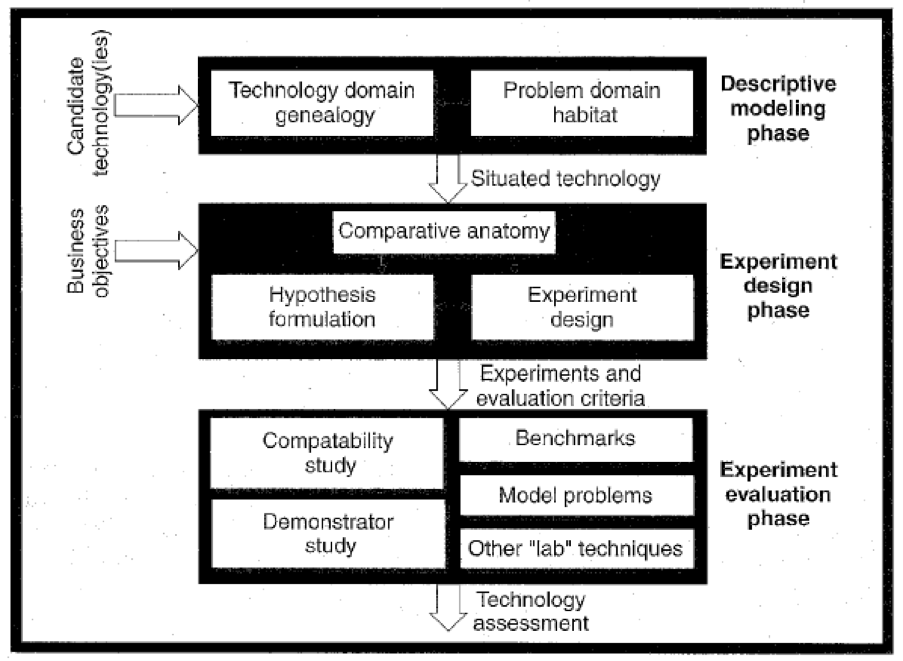
\includegraphics[scale=0.5]{figs/framework.png}
	\caption{Software technology evaluation framework.}
	\label{fig:framework}
\end{figure}

\subsection{Descriptive Modeling}

write where the technology comes from, its history, its context and what problem it solves.
Consider drawing a graph like in \cite{brown:96}.

We will now look into our different technologies more in depth.

\section{Origins and History of Kotlin} 

Source: \href{https://chatgpt.com/share/672e6c5a-aa64-8007-93e5-aefa60cbe9fc}{ChatGPT}
\\
\\
Kotlin was developed by JetBrains, the Czech software development company behind popular IDEs like IntelliJ IDEA. The name is derived from Kotlin Island, a Russian island in the Gulf of Finland, near St. Petersburg 
\href{https://en.wikipedia.org/wiki/Kotlin_(programming_language)}{Wikipedia}. JetBrains introduced Kotlin in 2011 as a modern programming language to address the limitations they experienced while working primarily with Java.

\subsection{Key Historical Milestones}
\begin{itemize}
    \item \textbf{2011}: Kotlin was officially announced by JetBrains.
    \item \textbf{2016}: The first stable version, Kotlin 1.0, was released after five years of development, gaining traction especially among Android developers.
    \item \textbf{2017}: Kotlin was adopted by Google as an official language for Android development, marking a significant milestone and boosting its popularity in the Android ecosystem.
    \item \textbf{2020}: JetBrains launched the Kotlin Foundation in collaboration with Google, further solidifying Kotlin's role in Android and JVM development.
    \item \textbf{Ongoing Development}: Kotlin continues to evolve, with recent versions focusing on multi-platform capabilities, enabling Kotlin to be used beyond JVM and Android (e.g., web, iOS, and server-side applications).
\end{itemize}

\section{Context and Ecosystem}

Kotlin is a statically typed programming language that compiles to Java bytecode and runs on the Java Virtual Machine (JVM), making it compatible with Java libraries and frameworks. Kotlin’s design emphasizes safety, conciseness, and interoperability with Java, which has made it particularly appealing in the following contexts:

\begin{itemize}
    \item \textbf{Android Development}: Kotlin is widely adopted in the Android ecosystem because it offers more concise syntax and better safety features than Java.
    \item \textbf{Server-Side Development}: Kotlin’s compatibility with Java allows it to integrate well with JVM-based server frameworks like Spring Boot.
    \item \textbf{Multi-Platform Development}: Kotlin/Native and Kotlin Multiplatform are expanding Kotlin's reach to other platforms, enabling shared codebases across mobile, web, and desktop applications.
\end{itemize}

\section{Problems Kotlin Solves}

\begin{itemize}
    \item \textbf{Verbosity in Java}: Java's verbosity can lead to long, repetitive code, especially for basic operations. Kotlin addresses this by introducing a more concise syntax that reduces boilerplate code.
    \item \textbf{Null Safety}: NullPointerExceptions (NPEs) are common in Java and can lead to runtime crashes. Kotlin provides built-in null safety, preventing many common NPEs by making developers explicitly handle nullable types.
    \item \textbf{Interoperability with Java}: Kotlin is fully interoperable with Java, allowing developers to gradually integrate Kotlin code into existing Java applications. This is ideal for teams looking to modernize their codebases without a full rewrite.
    \item \textbf{Improved Asynchronous Programming}: Kotlin’s coroutines offer a more streamlined way of handling asynchronous programming compared to Java’s standard concurrency options, making it easier to write non-blocking, concurrent code.
    \item \textbf{Multi-Platform Support}: Kotlin's multi-platform capabilities reduce duplication by allowing shared business logic across different environments, which is particularly beneficial for teams developing applications on multiple platforms.
\end{itemize}

\section{Visual Representation}

To visually illustrate Kotlin’s development and position relative to Java, we could represent Kotlin’s growth, with nodes highlighting key milestones like first stable release (2016), Google adoption for Android (2017), and expansion into multiplatform (ongoing).


\textbf{Backend:}

The reason we chose Kotlin with Spring Boot for this application is that Kotlin is compatible with Java and has many good features. Spring MVC also makes deploying a web application practical. Here are some of the features that Kotlin offers:

\begin{itemize}
    \item \textbf{Conciseness and Readability:} Kotlin syntax is more concise compared to Java, reducing redundant code. This makes the code easier to read and work with.
    
    \item \textbf{Null Safety:} Kotlin's type system helps eliminate null pointer exceptions, a common source of bugs in Java. Kotlin distinguishes between nullable and non-nullable types.
    
    \item \textbf{Interoperability:} Kotlin is fully interoperable with Java, allowing you to use existing Java libraries and frameworks without any issues.
    
    \item \textbf{Coroutines for Asynchronous Programming:} Kotlin's coroutines simplify asynchronous programming, making it easier to handle tasks that involve waiting for resources or events, such as network requests.
    
    \item \textbf{Extension Functions:} Kotlin allows you to extend existing classes with new functionality without modifying their code. This promotes cleaner code organization and better separation of concerns.
    
    \item \textbf{Data Classes:} Kotlin's data classes provide a simple way to create classes that are primarily used to hold data. They automatically generate useful methods like \texttt{equals()}, \texttt{hashCode()}, and \texttt{toString()}, simplifying data handling.
    
    \item \textbf{Higher-Order Functions and Lambdas:} Kotlin supports functional programming features, such as higher-order functions and lambda expressions, which can lead to more expressive and flexible code.
\end{itemize}


\subsection{Experiment Design}

Write you hypotheses about what benefits the technology bring and how you can support or reject them via experiments.

\subsection{Experiment Evaluation}

Write about the results of your experiments, either via personal experience reports, quantitative benchmarks, a demostrator case study or a combination of multiple approaches.


For some reports you may have to include a table with experimental
results are other kinds of tables that for instance compares
technologies. Table~\ref{tab:results} gives an example of how to create a table.

\begin{table}[bth]
	\centering
	\begin{tabular}{llrrrrrr}
		Config & Property & States & Edges & Peak & E-Time & C-Time & T-Time
		\\ \hline \hline
		22-2 & A   &    7,944  &   22,419  &  6.6  \%  &  7 ms & 42.9\% &  485.7\% \\
		22-2 & A   &    7,944  &   22,419  &  6.6  \%  &  7 ms & 42.9\% &  471.4\% \\
		30-2 & B   &   14,672  &   41,611  &  4.9  \%  & 14 ms & 42.9\% &  464.3\% \\
		30-2 & C   &   14,672  &   41,611  &  4.9  \%  & 15 ms & 40.0\% &  420.0\% \\ \hline
		10-3 & D   &   24,052  &   98,671  & 19.8  \%  & 35 ms & 31.4\% &  285.7\% \\
		10-3 & E   &   24,052  &   98,671  & 19.8  \%  & 35 ms & 34.3\% &  308.6\% \\
		\hline \hline
	\end{tabular}
	\caption{Selected experimental results on the communication protocol example.}
	\label{tab:results}
\end{table}
